\documentclass[10pt,journal,compsoc]{IEEEtran}

\usepackage[all,pdf]{xy}
\usepackage{tikz}




% *** CITATION PACKAGES ***
%
\ifCLASSOPTIONcompsoc
  % IEEE Computer Society needs nocompress option
  % requires cite.sty v4.0 or later (November 2003)
  \usepackage[nocompress]{cite}
\else
  % normal IEEE
  \usepackage{cite}
\fi

% *** MATH PACKAGES ***
%
\usepackage{amsmath}
\usepackage{amsthm}
\usepackage{todonotes}
\usepackage{nicefrac}
\usepackage{lmodern,amssymb}
\usepackage{float}
\usepackage{graphicx}
\usepackage{caption}
\usepackage{subcaption}
\usetikzlibrary{positioning}

\usepackage[utf8]{inputenc}
\usepackage[T1]{fontenc}
\usepackage[english]{babel}
\usepackage{pgfplots}

% Commands
\newcommand\smallO{
  \mathchoice
    {{\scriptstyle\mathcal{O}}}% \displaystyle
    {{\scriptstyle\mathcal{O}}}% \textstyle
    {{\scriptscriptstyle\mathcal{O}}}% \scriptstyle
    {\scalebox{.50}{$\scriptscriptstyle\mathcal{O}$}}%\scriptscriptstyle
  }

\interdisplaylinepenalty=2500


\newtheorem{theorem}{Theorem}
\newtheorem{lemma}{Lemma}
\newtheorem{definition}{Definition}

\hyphenation{op-tical net-works semi-conduc-tor}

\makeatletter
\def\endthebibliography{%
  \def\@noitemerr{\@latex@warning{Empty `thebibliography' environment}}%
  \endlist
}
\makeatother

\begin{document}

\title{Finding Lower Bounds for the Number of Comparison in Selection Algorithms}

\author{Josua Dörrer, Konrad Gendle, Johanna Hofmann, Julius von Smercek, Andreas Steding% <-this %
  \IEEEcompsocitemizethanks{\IEEEcompsocthanksitem Institut für Formale Methoden der
    Informatik (FMI)\protect\\
    Universität Stuttgart
  }}

\markboth{Bachelor-Forschungsprojekt}%
{Submission}

\IEEEtitleabstractindextext{%
  \begin{abstract}
    This research project aims to find worst case optimal comparison algorithms for selecting the
    i-th smallest of n elements of a set for n up to 15 with computer search.
  \end{abstract}

  \begin{IEEEkeywords}
    Selection, Pessimistic lower Bound, Partial Order Sets, Computer Search
  \end{IEEEkeywords}}


\maketitle

\IEEEdisplaynontitleabstractindextext


\IEEEpeerreviewmaketitle

\IEEEraisesectionheading{
  \section{Motivation}
  \label{sec:motivation}
} \IEEEPARstart{T}{he} problem of selecting the $i$-th smallest element in a list of $n$ elements is
a well known problem in computer science and called \textit{selection}. Explicitly, we
concern ourselves with optimal worst-case selection of a single element from a set of
initially unordered unique others, measuring the cost as number of comparisons made.
A first approach to solve
this can be achieved by sorting the list at first and selecting the $i$-th element. However, this
approach has a time complexity of $\mathcal{O}(n \cdot \log n)$. Putting more thought into this
problem one can find algorithms like the median of medians (Schöning \cite{Schoening1993}) or PICK
(Blum \cite{Blum1972}) and reduce the time complexity to $\mathcal{O}(n)$. Optimal algorithms are
known for any $n$ when $i$ is either one or two, but there is a significant performance gap finding
the median $i = \nicefrac{n}{2}$ from the best known algorithm with a time complexity of $2.97 \cdot
  n + \smallO(n)$ to the tightest known minimum of $2 \cdot n - \smallO(n)$.

Searching for optimal solutions is considerably difficult and the tightest known lower bounds
obtained by mathematical means soon exceed what is attainable by even rather intelligent search. An
approach to finding optimal algorithms is made by Gasarch, Kelly and Pugh \cite{Gasarch1996} who
introduced computer search to find optimal selection algorithms. On his website Kenneth Oksanen
\cite{Oksanen} published a computer search algorithm improving the previously known lower bounds
found by Gasarch et. al. However, the results are not published in a scientific journal and lack
explanation. This work will continue the work of Oksanen \cite{Oksanen} by confirming, improving and
expanding the values he found. It will reimplement some ideas of the algorithms Oksanen published
along with his found lower bounds and improve the computer search algorithms by researching the
benefits of different search strategies, adding $\alpha$-$\beta$-pruning and the exploitation of
compatible Posets. A quote from Miguel de Cervantes from Don Quijote will hold true for this
article: The journey is better than the inn. So buckle up.

\section{Fundamentals}
\subsection{Algorithms for Finding the $i$-th largest of $n$ elements}
\subsubsection{Sorting}
A baseline algorithm to select the $i$-th element in a list of $n$ values is to use a sorting
algorithm like merge sort or heap sort on the input data and then return the $i$-th element of the
now sorted list. The time complexity of this approach is essentially the runtime to sort the list.
For the sorting algorithms mentioned the time complexity is of $\mathcal{O}(n \cdot \log n)$

\subsubsection{Pivoting}
A better approach solving the selection problem can be achieved by using pivoting. The common idea
of the algorithms using pivoting is to promote an element from the input to a so called
\textit{pivot} element and use comparisons against this element to divide the remaining $n-1$ input
elements into two subsets. Let $L$ be the subset with elements less then the pivot element and $G$
the subset with elements greater than the pivot element. The algorithm can then determine whether to
search for the $i$-th element in the subset $L$ or the subset $G$. Using pivot algorithms like
Floyd-Rivest algorithm, a variation of quickselect, the runtime can be reduced to
$\mathcal{O}(\sqrt{n \cdot \log n})$. The first linear-time deterministic selection algorithm known
is  also commonly taught in computer science class is the median of medians. It partitions the input
data into sets of five in linear time. Then it calls itself on each of the sets to find the median
of these sets of five. The result is a algorithm that returns the median in $\mathcal{O}(n)$. In
practice the algorithm performs poorly compared to quickselect and is also slower than sorting the
list of moderate size due to its high constant factor. Better algorithms like quickselect or PICK
have a lower constant factor but all these algorithms share the same time complexity
$\mathcal{O}(n)$.
\todo{hier fehlt ein cite}
% https://en.wikipedia.org/wiki/Selection_algorithm#cite_note-knuth-14

\subsubsection{Lower and upper bounds}
The time complexity of $\mathcal{O}(n)$ of the mentioned algorithms is inevitable, because the input
to these algorithm is a list of values in arbitrary order. Therefore, the algorithm must look at all
the input values to determine a correct solution. If any of these input values will not be
considered it could be the one that should have been returned by the algorithm leading to wrong
results. Apart from this simple and straightforward argument, there is a considerable amount of
research on the exact number of comparisons required for selection, both in the randomized and
deterministic cases.

It has been found that selecting the $i$-th element of $n$ requires at least
$n+\min(i,n-i)-\mathcal{O}(1)$ comparisons, thus matching the average case of the Floyd-Rivest
algorithm up to his $\smallO(n)$ term. For deterministic algorithms it has also been shown that
\begin{eqnarray*}
  &\left (1 + H(i/n) \right ) \cdot n + \Omega(\sqrt n) \\
  &\text{with~} H(x) = x \cdot \log_2 \frac{1}{x} + (1-x) \log_2 \frac{1}{1-x}
\end{eqnarray*}
are required. An upper bound is been proposed by Blum, in the paper \textit{Time Bounds for
  Selection}. It stated that no more than $5.430\dot{5} \cdot n$ comparisons are ever required.
Therefore selection is for sure in a time complexity of $\mathcal{O}(n)$ for best and worst-case.

\begin{lemma}
  If $k$ is a lower bound for selecting $i$ of $n$, then selecting $i$ of $n+1$ must take at least $k+1$ comparisons.
\end{lemma}
\begin{proof}
  Assume some algorithm exists that selects $i$ of $n+1$ in $k$ comparisons. It must have two elements it compares first.
  If we input a by definition largest element in place of one of them the algorithm must still return the correct $i$-th
  largest of the remaining $n$ elements. But because this element is larger by definition, the first comparison may be 
  skipped, thus reducing the number of comparisons by at least 1. Thus taking out all occurrences of that element will 
  yield an algorithm for $i$ of $n$ in $k-1$ comparisons, which contradicts the condition of $k$ being a lower bound.
\end{proof}

\subsection{Partial Order Sets}
To dive deeper into these algorithms the concept of partial orders needs to be introduced. A partial
order is an ordering relation
$\leq$ on a set $P$ that satisfies reflexivity, anti symmetry, and transitivity. 

\begin{definition}[Selection Poset]
  Given a set of elements $\Omega$ with $|\Omega| = n < \infty$ we write 
  $(n, i, R)$ for the selection of the $i$-th largest of $n$ elements
  with the existing comparisons $R$.
  Explicitly, $R\subseteq\Omega^2$ such that $(a, b)\in R \Longleftrightarrow a \leq b$.

  The enumeration of $i$ starts at $0$, so $(4, 1, R)$ is the second smallest,
  rather than the minimum.
\end{definition}

The SELECT problem is thus embedded as $(n, i, \emptyset)$.

\begin{definition}[Reduced]
  A poset is \textbf{Reduced} if all of its elements have less than $i-1$ elements smaller than themselves and less than $n-1$ larger. Hence, all elements are still possible solutions.
\end{definition}
\begin{definition}[Canonified]
  A poset \textbf{Canonified} if it matches the following conditions making it unique among all posets isomorphic to it.

  Some parts of this paper use a best effort
  approximation for this to increase speed, the results are then called \textbf{Pseudo Canonified}.
\end{definition}
\begin{definition}[Normal]
  A \textbf{Normal} poset is reduced and canonified.
\end{definition}

\begin{definition}[Optimal Cost]
  The cost $V(P)$ of the poset $P = (n, i, R)$
  is the optimal number of further comparisons needed to
  perform the selection.

  We measure this pessimistically, meaning that among all
  possible outcomes of those further comparisons we assume
  the most expensive ones.
\end{definition}

\begin{definition}[Inverse poset] \label{definition:inverse_poset}
  The inverse of a poset $P=(n, i, R)$ is the poset $P^{-1}=(U,R',n-1-i)$ with $R' = \{(u,v) \; \vert \; (v,u) \in R\}$.
\end{definition}

\begin{lemma}
  For a given poset $P = (n, i, R)$ $V(P) = V(P^{-1})$
\end{lemma}

\begin{proof}
  Given $V(P)$, we know that we can construct an algorithm that
  solves $P$ in exactly that many comparisons, i.e. it determines
  the element with exactly $i-1$ less and exactly $n-i$ greater
  than itself.

  Since $n$ and $i$ are fixed, this algorithm can be converted into
  a binary decision tree and by swapping all the children, the new 
  algorithm must now select the element such that $n-i$ are smaller 
  and $i-1$ are larger than it while assuming an inverted $R$, which is 
  the solution for $P^{-1}$. 
\end{proof}

%[\todo{cite:https://en.wikipedia.org/wiki/Partially_ordered_set}]

\subsubsection{Solved Posets and Compatible Solutions}
By definition of the problem, we seek an
element that is larger than $n-i$ elements and smaller than
$i-1$ elements. 

\begin{lemma}
  Solving a poset requires knowing the explicit elements
  making up these two sets.
\end{lemma}
\begin{proof}
  Suppose we have determined the element $e$ to be the 
  solution, and an element $p$ unordered with $e$.

  Then $p$ may be above as well as below $e$, which
  can't be the solution in both cases.
\end{proof}

\begin{definition}[Compatible Solution]
  As such we can define a \textbf{Compatible Solution} $Q = (n, i, S), |S|=n-1$ of a poset $P=(n, i, R)$,
  similar to the concept of linear extensions for
  regular posets %[todo cite]
  , to be solved, and $(a, b)\in S\implies (b, a)\notin R$.
\end{definition}

Let $P = (U, B, i)$ be a reduced poset, where elements which cannot be the solution are removed.
Let $Q = (U, C, i)$ be a poset with an element $u \in U$, where $i$ elmenets are smaller than $u$ and $n-i-1$ elements are larger than $u$.
Every comparison $(a,b) \in C$ in $Q$ compares an element to $u$, meaning either $a = u$ or $b = u$.

We call $Q$ compatible with $P$ if no comparison in $Q$ contradicts a comparison in $P$; meaning for all comparisons $(a,b) \in C$ it should hold that $(b,a) \not\in B$.
Let $$\mathcal{C}(P) = \{Q \mid Q \text{ compatible with } P\}$$ be the set of all posets compatible with $P$.

We conjecture that a poset $P$ is always solvable in $\lceil\log_2(|\mathcal{C}(P)|)\rceil$ or less comparisons.


\subsection{Example}
\begin{figure}[h!]
  \centering
  \begin{tikzpicture}[tcancel/.append style={draw=#1, cross out, inner sep=6pt}]
  \draw(-.5, -.5) rectangle (4.5, .5);
  \node[circle,draw=black] (A1) at (0, 0) {};
  \node[circle,draw=black] (A2) at (1, 0) {};
  \node[circle,draw=black] (A3) at (2, 0) {};
  \node[circle,draw=black] (A4) at (3, 0) {};
  \node[circle,draw=black] (A5) at (4, 0) {};

  \draw[dashed] (A1) -- (A2) node {};
  \draw[dashed] (A3) -- (A4) node {};

  \draw(-0.5, -3.0) rectangle (4.5, -1.0);
  \node[circle,draw=black] (B1) at (1.0, 0 - 2.5) {};
  \node[circle,draw=black] (B2) at (1.0, 1 - 2.5) {};
  \node[circle,draw=black] (B3) at (2.0, 0 - 2.5) {};
  \node[circle,draw=black] (B4) at (2.0, 1 - 2.5) {};
  \node[circle,draw=black] (B5) at (4.0, 0.5 - 2.5) {};

  \draw (B1) -- (B2) node {};
  \draw (B3) -- (B4) node {};
  \draw[dashed] (B2) -- (B4) node {};

  \draw(-0.5, -6.0) rectangle (4.5, -3.5);
  \node[circle,draw=black] (C1) at (1, 0 - 5.5) {};
  \node[circle,draw=black] (C2) at (1, 1 - 5.5) {};
  \node[circle,draw=black,tcancel=red] (C3) at (2, 1.5 - 5.5) {};
  \node[circle,draw=black] (C3) at (2, 1.5 - 5.5) {};
  \node[circle,draw=black] (C4) at (2, .5 - 5.5) {};
  \node[circle,draw=black] (C5) at (3, .5 - 5.5) {};

  \draw (C1) -- (C2) node {};
  \draw (C3) -- (C4) node {};
  \draw (C2) -- (C3) node {};
  \draw[dashed] (C4) -- (C5) node {};

  \draw(-0.5, -8.5) rectangle (4.5, -6.5);
  \node[circle,draw=black] (D1) at (1.0, 0 - 8) {};
  \node[circle,draw=black] (D2) at (1.0, 1 - 8) {};
  \node[circle,draw=black] (D3) at (2.0, 0 - 8) {};
  \node[circle,draw=black] (D4) at (2.0, 1 - 8) {};
  \node[circle,draw=black,tcancel=red] (D5) at (4.0, 0.5 - 8) {};
  \node[circle,draw=black] (D5) at (4.0, 0.5 - 8) {};

  \draw (D1) -- (D2) node {};
  \draw (D3) -- (D4) node {};
  \draw[dashed] (D2) -- (D4) node {};

  \draw(-0.5, -11.5) rectangle (4.5, -9.);
  \node[circle,draw=black,tcancel=red] (E1) at (1, 0 - 11.0) {};
  \node[circle,draw=black] (E1) at (1, 0 - 11.0) {};
  \node[circle,draw=black] (E2) at (1, 1 - 11.0) {};
  \node[circle,draw=black,tcancel=red] (E3) at (2, 1.5 - 11.0) {};
  \node[circle,draw=black] (E3) at (2, 1.5 - 11.0) {};
  \node[circle,draw=black] (E4) at (2, .5 - 11.0) {};
  \node[circle,draw=black,tcancel=red] (E5) at (3, .5 - 11.0) {};
  \node[circle,draw=black] (E5) at (3, .5 - 11.0) {};

  \draw (E1) -- (E2) node {};
  \draw (E3) -- (E4) node {};
  \draw (E2) -- (E3) node {};
  \draw[dashed] (E2) -- (E4) node {};
\end{tikzpicture}
  \caption{Finding the median $i=2$ of $n=5$ values using six comparisons.}
  \label{fig:median_of_5}
\end{figure}
A good visual example is finding the median $i=2$ in a list of $n=5$ elements. Figure
(\ref{fig:median_of_5}) illustrate the search of the median using Hasse diagrams. Each step shows
the comparisons to be performed next as a yellow line. A Hasse diagram of the order of relation
found so far (smaller=lower, larger=higher) is shown as the blue lines. The red circles have already
found to be greater than three others and disqualified The red elements have already been determined
to be larger than three other elements and are therefore disqualified as medians. The larger
element of the final comparison is the median. This is also the optimal algorithm for $i=2$ and
$n=5$.


\section{Methods and Tools}
In this section we describe our three main approaches being the forward search, backward search and bidirectional search. Furthermore, we explain how we harness the notion of compatible posets with respect to all of the three search approaches.

\subsection{Forward Search}\label{chapter:forward_search}
Forward Search starts with an empty Poset, i.e. one with entirely unknown ordering of its elements,
and recursively determines solvability of a given Poset within some bound by exhaustively searching
the results of all possible comparisons to be made unless it is already solved or we determine that
it cannot be solved within the alloted number of comparisons by some heuristic.

Between the two possible outcomes of a comparison we assume the worse, but since an algorithm is
free to choose which elements to compare we are looking for the most useful comparison, the one that
yields result Posets cheapest to solve themselves, still in terms of worst case outcome. The
algorithms output by the search program are built by saving the comparison that lead to this
cheapest to solve result.

To limit memory cost and allow further pruning we traverse the search tree depth first, reducing the
maximum number of comparisons alloted to child Posets to one less than the current best result
found. This premise is implemented by Minimax algorithms as shown in
figure~\ref{fig:minimax_search}.

We can drastically speed up this exploration by caching previous results, even with a simple usage
based ejection policy. Since the search always imposes an upper bound for the number of comparisons
to allow this also includes yet unsolved Posets, for which we note the currently known minimum.

The minimax search algorithm also allows for cutting off unpromising branches. For this means, and inspired by the idea of $\alpha$-$\beta$-pruning, two strategies are applied.
Firstly, we use a socalled solvable-heuristic.
The heuristic is employed to estimate whether a poset is solvable. If the heuristic's estimate states 'unsolvable', the branch is pruned.
Otherwise, the search continues regularly.
Secondly we use a measure called \texttt{current\_best}.
Each call of \texttt{search\_rec} gets a maximum numbers of comparisons. When searching the children of a node, the limit is the best (minimal) value found so far.

It is optimal because of an inductive argument over the number of relative orders determined. An
already solved Poset obviously takes no further comparisons to solve. Then, given an unsolved Poset
with all elements already too large or small excluded we must make at least one more comparison to
make progress. Since all Posets resulting from these comparisons must have more elements ordered
than the current one has we can assume as per induction that we know their optimal cost. As a result, we
cannot solve the Poset in less than the cost of the cheapest of these comparisons, plus one for the
comparison itself, hence the current Poset is also solved optimally.

It is also complete for a given upper bound, explainable through a similar inductive argument. If
the Poset is solvable within that bound, then at least one of its possible comparisons must have both
outcomes be solvable within the bound lowered by one. Since the search only lowers the bound imposed
on its recursive descendants beyond that once at least one has been solved, we are also guaranteed
to find a solution for the original Poset if it exists within the bound.

\begin{figure}
  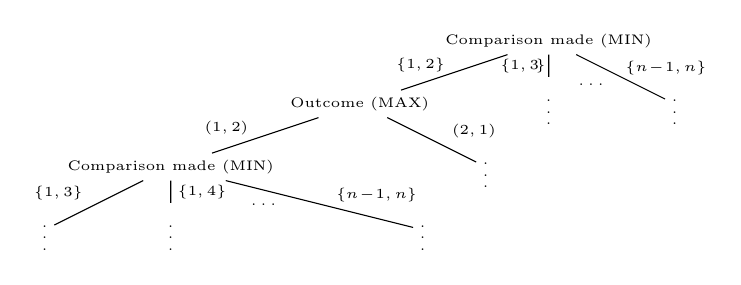
\begin{tikzpicture}[scale=0.8]
  \tiny
  \node (A1) at (0,0) {$\vdots$};
  \node (A2) at (2,0) {$\vdots$};
  \node (A3) at (3.5,0.4) {$\dots$};
  \node (A4) at (6,0) {$\vdots$};

  \node (B1) at (2,1) {Comparison made (MIN)};

  \draw (B1) -- (A1) node[above,pos=0.6, xshift=-0.4cm] {$\{1,3\}$};
  \draw (B1) -- (A2) node[right, midway] {$\{1,4\}$};
  \draw (B1) -- (A4) node[right, pos=0.3, xshift=6mm] {$\{n \!- \! 1,n\}$};

  \node (C1) at (5,2) {Outcome (MAX)};
  \node (B2) at (7,1) {$\vdots$};

  \draw (C1) -- (B2) node[right, pos=0.3, xshift=4mm] {$(2,1)$};

  \draw (B1) -- (C1) node[left, pos=0.7, xshift=-4mm] {$(1,2)$};

  \node (D1) at (8,3) {Comparison made (MIN)};
  \node (C2) at (8,2) {$\vdots$};
  \node (C3) at (8.7,2.3) {$\dots$};
  \node (C4) at (10,2) {$\vdots$};

  \draw (D1) -- (C1) node[left,pos=0.3,xshift=-3mm] {$\{1,2\}$};
  \draw (D1) -- (C2) node[left, midway, xshift=0.5mm] {$\{1,3 \! \}$};
  \draw (D1) -- (C4) node[right, pos=0.3,xshift=2mm] {$\{n \! - \! 1,n\}$};

\end{tikzpicture}
  \caption{Minimax search algorithm}
  \label{fig:minimax_search}
\end{figure}

\subsubsection{Canonification}

When caching the posets we have to check, whether two posets are isomorphic to eachother.
We consider a poset isomorphic to another poset if we can relabel the elements of one poset to obtain the other poset.
This problem is expensive to solve for every poset comparison.

After adding a comparison to a poset, we transform the poset to a canonical form.
All posets, that are isomorphic to eachother should be transformed to the same canonical form.
Computing the canonical form can be done using Nauty, but this takes a significant amount of time.
Some performance tests show that it is faster to compute an almost canonical form, where some posets that are isomorphic to eachother result in different canonified forms.
As a result, some posets that are isomorphic occupy several cache entries, but canonifying a poset is much faster.

\subsection{Backward Search} \label{sec:backward}

Backward search starts with a solved poset, then repeatedly attempts to remove comparisons from its
frontier posets such that the same poset with the opposite comparison result is also found within
those already discovered.

Thus, the number of iterations taken until a poset is added to the frontier equals the number of
worst case comparisons needed to solve it, which means that the search terminates once the empty
poset with the desired $n$ and $i$ is found.

The argument for correctness is that the number of comparisons for which we have found all posets solvable within them equals the number of iterations of the search.
If for a given poset and a comparison within it we have already discovered both results then their cost must be less than the current number of iterations. Hence, we can conclude that the poset is solvable within this number of comparisons.
Since this condition did not hold true in any previous iteration, we can further infer that the cost must also be optimal.
And if a poset is solvable within
that number of comparisons it must have at least one comparison with a result among the Posets
discovered in the previous iteration, as otherwise it would have to be solvable in less.

%%%%%%%%%%%%%%%%%%%%%%%%%%%%%%%%%%%%%%%%%%%%%%%%%%%%%%%%%%%%%%%%%
% TODO: In Papern suche, ob die Rückwärtssuche wirklich komplett neues Gebiet ist

% TODO: @Johanna: ab hier übersetzen :)

\subsubsection{Normal Form} \label{sec:backward:normal_form}

In contrast to the forward search, the backward search uses a unique canonicalization.
The canonicalization of the forward search is not unique for performance reasons.

\subsubsection{Normalform}
Note that the backward search requires a unique normal form. In case our custom canonification does not yiel a unique form, nauty provides the proper canonification.
In the following, the canonification process is explained.

First, it is determined whether $i < n-1-i$ holds.
If this does not hold true, $P$ is replaced by $P^{-1}$.
According to lemma~\ref{lemma:inverse_poset} the poset's solvability remains unaltered.

Finally, the poset's elements are aranged canonically. 
As a means to this end, the poset is represented as a directed graph with respect to its Hasse diagram.
The canonic labelling of the elements is provided by nauty, which is a programm in C for the calculation of graph automorphism groups \cite{MCKAY201494}.
With this canonic labelling the poset can be portrayed canonically.
A potential problem occurs, if $i = n - 1 - i$ holds.
In this case, it is impossible to decide whether $P$ or $P^{-1}$ corresponds to
to the canonical normal form based on the value of $i$.

\begin{figure}
  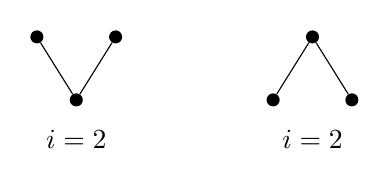
\begin{tikzpicture}
  \node[circle,fill=black,scale=0.5] (A1) at (1, 0) {};
  \node[circle,fill=black,scale=0.5] (A2) at (0.5, 0.8) {};
  \node[circle,fill=black,scale=0.5] (A3) at (1.5, 0.8) {};

  \draw (A1) -- (A2) node {};
  \draw (A1) -- (A3) node {};
  \node (AL) at (1, -0.5) {$i = 2$};


  \node[circle,fill=black,scale=0.5] (B1) at (3 + 1, 0.8) {};
  \node[circle,fill=black,scale=0.5] (B2) at (3 + 0.5, 0) {};
  \node[circle,fill=black,scale=0.5] (B3) at (3 + 1.5, 0) {};

  \draw (B1) -- (B2) node {};
  \draw (B1) -- (B3) node {};
  \node (BL) at (3 + 1, -0.5) {$i = 2$};
\end{tikzpicture}
  \centering
  \caption{Problematischer Fall}
  \label{fig:backward_canonify_problematic}
\end{figure}

In the Hasse diagram in figure~\ref{fig:backward_canonify_problematic} the posets appear unidentical, despite them being each others inverse.
To mitigate th
In order to eliminate this ambiguity, the inverse is also calculated and canonicalized for each poset for which $i = n - 1 - i$ applies.
One of the two is then selected deterministically.

Since canonification is inevitable for the backward search but takes up a large portion of the computing time, all trivial cases are treated manually and only the remaining cases are canonified by nauty.

The manual cononification works as follows. 
First, the in- and outdegree is calculated for aeach nodes. 
Based on these values a hash value is assigned to each node.
The hash also takes into account the topological structure of all adjacent nodes recursively upto a certain recursion depth limit.

Then, the nodes are sorted according to their in- and outdegree and their hash value.
If each degree and each hash value is unqiue the graph finally attained its unique normal form.
For two nodes having identical attributes, it is attempted to swap them.
If the representation remains unchanged, the poset is regarded as uniquely canonified, since both graphs map to the same representation. 
If the representations differ, the graph is treated as follows. 
Let there be $l$ pairs of nodes with the same attributes, respectively.
The algorithm iterates over all possible permutations.
For the first pair there are two possibilites: Either the nodes are swaped, or they remain unchanged.
Under the realistic assumption of $l$ being small, all possible $2^l$ possible permutations can be efficiently iterated.
Finally, one permutation is selected deterministically based on its representation.

Applying this canonification preprocessing reduces the cases requiring nauty drastically, as shown in table~\ref{table:nauty-ratio} for $n=13$.

It is particularly noteworthy that for higher $i$, the percentage of nauty calls declines.
For small values of $i$, the high percentage of nauty is uncritical, as the result for small $i$ can be calculated quickly anyway.
\begin{table}
  \begin{tabular}{l|l}
    $i$ & nauty-Ratio \\
    \hline
    $0$ & $0.000\%$   \\
    $1$ & $30.205\%$  \\
    $2$ & $6.797\%$   \\
    $3$ & $1.530\%$   \\
    $4$ & $0.469\%$   \\
    $5$ & $0.188\%$   \\
    $6$ & $0.116\%$
  \end{tabular}
  \centering
  \caption{Prozentuale Häufigkeit der Aufrufe von nauty zur Kanonisierung für $n = 13, i = 6$}
  \label{table:nauty-ratio}
\end{table}

\subsubsection{Algorithmus} \label{sec:backward:algorithm}
% Schreibweise: $\text{P}^{n, i}$
% select(n, i)

Die Eingabe für die Rückwärtssuche sind die Parameter $n$ und $i$.
Die Rückwärtssuche beginnt mit dem kleinsten gelösten Poset und berechnet iterativ alle Posets, die in $1, 2, 3, \dots$ Vergleichen gelöst werden können, bis das leere Poset mit $n$ Elementen und dem $i$-kleinsten gesuchten Element gefunden wird.
Das kleinste gelöste Poset besteht aus einem Element und enthält keine Vergleiche.
Das leere Poset besteht aus $n$ Elementen, wobei das $i$-kleinste Element gesucht wird, und beinhaltet keinen Vergleich.
Allgemein sei $A_k$ die Menge aller Posets, die in $k$ Vergleichen lösbar sind.
$A_0$ besteht nur aus dem kleinsten gelösten Poset.
Im Folgenden berechnet die Rückwärtssuche für jedes Poset in der Menge $A_k$ die entsprechenden Vorgänger.
Die Menge aller Vorgänger bildet die Menge $A_{k + 1}$.
Wenn das leere Poset mit $n$ Elementen und dem $i$-kleinsten gesuchten Element in $A_l$ vorhanden ist, werden genau $l$ Vergleiche benötigt, um das $i$-kleinste Element einer $n$-elementigen Liste zu bestimmen.

\subsubsection{Vorgängerberechnung} \label{sec:backward:predecessor_calculation}

\begin{definition}[Vorgänger] \label{definition:predecessor_calculation}
  Poset $q$ ist Vorgänger von Poset $p$, wenn folgende Eigenschaften gelten:
  \begin{itemize}
    \item $q$ ist reduziert und eindeutig kanonisiert.
    \item $q$ wurde in keiner vorherigen Runde gefunden (da es sonst in weniger Vergleichen lösbar wäre).
    \item Es existiert ein Vergleich $(i, j)$, durch dessen Hinzunahme in $q$ und anschließende Normalisierung wieder das Poset $p$ resultiert und durch Hinzunahme des umgekehrten Vergleichs $(j, i)$ und anschließende Normalisierung ein bereits gefundenes Poset resultiert.
  \end{itemize}
\end{definition}

\begin{lemma} \label{lemma:predecessor_calculation}
  Wenn Poset $p$ in $k$ Vergleichen lösbar ist und $q$ ein Vorgänger von Poset $p$ ist, ist Poset $q$ in $k + 1$ Vergleichen lösbar
\end{lemma}

\begin{proof} \label{proof:predecessor_calculation}
  Da $q$ in keiner vorherigen Runde gefunden wurde, ist es gemäß Annahme nicht in weniger Vergleichen lösbar.
  Da ein Vergleich $(i, j)$ existiert, durch dessen Hinzunahme und anschließende Normalisierung das Poset $p$ resultiert, kann $q$ durch die Hinzunahme eines Vergleichs erreicht werden.
  Da $p$ in $k$ Vergleichen lösbar ist, ist somit $q$ in $k + 1$ Vergleichen lösbar.
  Wenn der Vergleich umgekehrt eingefügt wird, befindet sich das resultierende Poset, gemäß Annahme, bereits im Cache.
  Dadurch ist dieser Pfad in höchstens $k + 1$ Vergleichen lösbar.
\end{proof}

Da potenziell unendlich viele Vorgänger existieren, werden diese nur bis zu einer maximalen Grenze von $n_{\text{max}}$ Elementen berechnet.
Die Berechnung eines Vorgängers für ein gegebenes Poset $p$ mit $n$ Elementen, bei dem das $i$-kleinste Element gesucht wird, erfolgt in drei Schritten:

\begin{itemize}
  \item[1.]
    Zunächst werden alle Posets mit $n$ Elementen gesucht, die durch das Einfügen eines Vergleichs, gefolgt von der Kanonisierung, wieder in Poset $p$ resultieren.

    Eine Schwierigkeit stellen die transitiven Vergleiche dar, da durch das Einfügen eines Vergleichs mehrere Vergleiche miteingefügt werden können.

    \begin{figure}
      \centering
      \begin{tikzpicture}
  \node[circle,draw=black] (A1) at (0, 0) {};
  \node[circle,draw=black] (A2) at (0, 1) {};
  \node[circle,draw=black] (A3) at (0, 2) {};

  \draw (A1) -- (A2) node {};
  \draw (A2) -- (A3) node {};
  \node (AL) at (0, -0.5) {$i = 1$};
  \node (A) at (0, -1) {(1)};


  \node[circle,draw=black] (B1) at (2.5 + 0, 0) {};
  \node[circle,draw=black] (B2) at (2.5 + 0, 2) {};
  \node[circle,draw=black] (B3) at (2.5 + 1, 1) {};

  \draw (B1) -- (B2) node {};
  \node (BL) at (2.5 + 0.5, -0.5) {$i = 1$};
  \node (B) at (2.5 + 0.5, -1) {(2)};


  \node[circle,draw=black] (C1) at (5 + 1, 2) {};
  \node[circle,draw=black] (C2) at (5 + 0, 0) {};
  \node[circle,draw=black] (C3) at (5 + 2, 0) {};

  \draw (C1) -- (C2) node {};
  \draw (C1) -- (C3) node {};
  \node (CL) at (5 + 1, -0.5) {$i = 1$};
  \node (C) at (5 + 1, -1) {(3)};
\end{tikzpicture}
      \caption{Problematischer Fall mit transitiven Vergleichen}
      \label{fig:backward_problematic}
    \end{figure}

    Wie in Abbildung~\ref{fig:backward_problematic} veranschaulicht, sind alle drei Posets vollständig reduziert und kanonisiert.
    Durch das Einfügen eines Vergleichs in Poset (2) oder in Poset (3) kann beide Male Poset (1) resultieren.
    Das bedeutet, dass je nach aktuellem Cache Poset (2) und Poset (3) potentielle Vorgänger sind, obwohl beide Male der gleiche Vergleich eingefügt wird.

    Um dieses Problem zu lösen, werden alle potentiellen Vorgänger berechnet.

  \item[2.]
    Im nächsten Schritt werden alle Vorgänger berechnet, die $n + 1$ Elemente haben und durch Einfügen eines Vergleichs gefolgt von einer Kanonisierung erneut das Poset $p$ ergeben.

    Da das neue Element kleiner oder größer als das gesuchte $i$-kleinste Element ist, wird bei diesen Vorgängern nach dem $i + 1$-kleinsten bzw. dem $i$-kleinsten Element gesucht.
    Da das Poset $p$ kanonifiziert ist, gilt $i \leq n - 1 - i$ für $p$.
    Durch das Kanonifizieren des Posets mit $n + 1$-Elementen und dem $(i + 1)$-kleinsten gesuchten Element, kann es hier jedoch nötig sein das Inverse Poset zu bilden wodurch das $(n + 1) - (i + 1) - 1 = n - i + 1$-te Element gesucht ist.

    Hierfür wird in Poset $p$ ein neues Element sowie passende Vergleiche eingefügt.
    Passende Vergleiche bedeutet, dass das neue Element nicht unmittelbar wegreduziert werden darf und es noch einen Vergleich gibt, der eingefügt werden könnte, ohne dass das neue Element wegreduziert werden kann, nach Lemma~\ref{lemma:remove_only_last_element_edge}.

    \begin{lemma} \label{lemma:remove_only_last_element_edge}
      Um alle möglichen Vorgänger mit $n + 1$ Elementen zu konstruieren, müssen nur Vergleiche zwischen dem neuen Element und beliebig vielen anderen Elemente hinzugefügt werden.
    \end{lemma}

    \begin{proof} \label{proof:remove_only_last_element_edge}
      Angenommen, es existiert ein Vorgänger mit $n + 1$ Elementen, bei dem das $(n + 1)$-te Element wegreduziert werden kann, wenn ein Vergleich zwischen dem $i$-ten und dem $j$-ten Element eingefügt wird, wobei $0 \leq i < j \leq n$.
      Dann ... % TODO: idk
    \end{proof}

    Anschließend werden die Posets aus dem 1. und 2. Schritt in einer Menge zusammengeführt und es wird sichergestellt, dass alle Posets kanonisiert sind.
    Bezeichne den Vergleich, der eingefügt werden könnte, ohne das ein Element wegreduziert werden kann im folgenden als den entfernten Vergleich.

  \item[3.]
    Im dritten Schritt wird für jedes bereits gefundene Element iterativ neue Elemente eingefügt, bis die obere Grenze $n_{\text{max}}$ erreicht ist.
    Wenn ein neues Element eingefügt wird, muss beachtet werden, dass eventuell nicht mehr das $i$-kleinste, sondern das $(i + 1)$-kleinste Element gesucht wird, genau wie im 2. Schritt, und das neue Element nicht direkt wegreduziert werden kann.
    Des Weiteren muss durch das Einfügen im 1. und 2. Schritt entferten Vergleichs und anschließendem reduzieren sowie kanonifizieren wieder Poset $p$ resultieren.

  \item[4.]
    Im letzten Schritt wird für jeden Vorgänger die minimale Anzahl an Vergleichen berechnet, die noch entfernt werden müssen, bis das leere Poset erreicht ist.
    Diese Anzahl entspricht den Kanten im zugehörigen Hasse-Diagramm.
    Anhand der bekannten theoretischen oberen Schranken können alle Posets verworfen werden, die zu viele Vergleiche enthalten, da diese zu keinem leeren Poset in den verbleibenden Vergleichen führen können und somit auch in der Vorwärtssuche nicht betrachtet werden können.
\end{itemize}

Da die theoretischen oberen Schranken in der Praxis zu hoch sind, verwendet das Programm einen iterative deepening-Ansatz.
Dieser beginnt mit einer oberen Grenze, die der theoretischen unteren Schranke entspricht, und erhöht diese Grenze iterativ, bis schließlich eine Lösung gefunden wird.
Obwohl dieser Ansatz dazu führt, dass die Rückwärtssuche mehrfach neu gestartet wird, da keine Ergebnisse aus vorherigen Runden übernommen werden können, kann dadurch der Suchraum erheblich eingeschränkt werden.

% TODO: Hier muss ein Bild vom Suchbaum hin für z.B. 4,1 (also schöner)
\begin{figure}[h!]
  \centering
  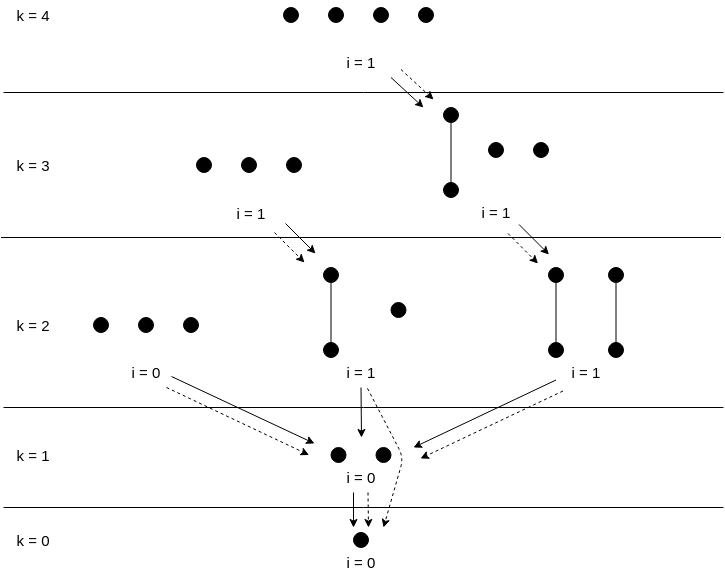
\includegraphics[width=\columnwidth]{figures/backward-search-tree.png}
  \caption{Suchbaum für $n = 4, i = 1$, k gibt Anzahl Vergleiche}
  \label{fig:backward-search-tree}
\end{figure}

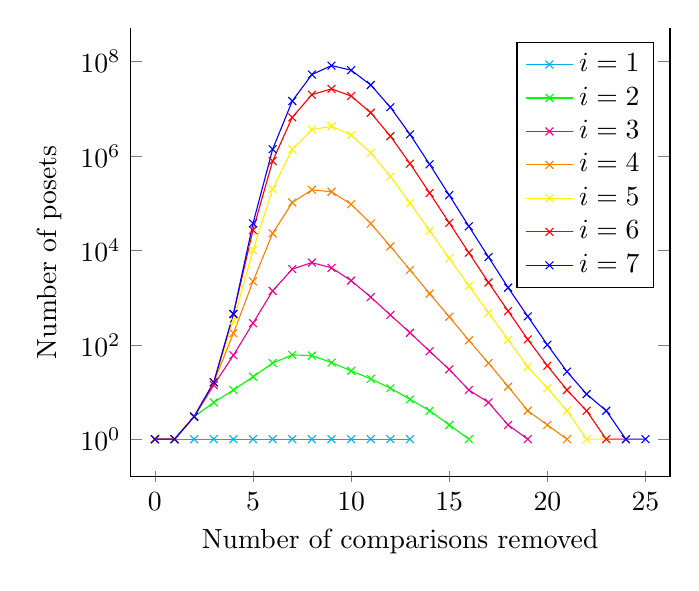
\begin{tikzpicture}
  \begin{axis}[
      ymode=log,
      axis x line = bottom,%x-Achse nur unten
      % x dir=reverse,
      enlarge x limits = .05,%x-Achse erweitern
      x axis line style = {-},%kein Pfeil
      % title = {\dots},
      ylabel={Number of posets},
      xlabel={Number of comparisons removed},
      % only marks,
      cycle list={{mark=x}},
      legend pos=north east,
    ]
    \addlegendentry{$i = 1$}
    \addplot+[cyan] table { %n=14,i=0
        x  y
        0  1
        1  1
        2  1
        3  1
        4  1
        5  1
        6  1
        7  1
        8  1
        9  1
        10 1
        11 1
        12 1
        13 1
      };
    \addlegendentry{$i = 2$}
    \addplot+[green] table { %n=14,i=1
        x y
        0  1
        1  1
        2  3
        3  6
        4  11
        5  21
        6  41
        7  61
        8  59
        9  42
        10 28
        11 19
        12 12
        13 7
        14 4
        15 2
        16 1
      };
    \addlegendentry{$i = 3$}
    \addplot+[magenta] table { %n=14,i=2
        x y
        0  1
        1  1
        2  3
        3  14
        4  60
        5  287
        6  1385
        7  4005
        8  5510
        9  4268
        10 2284
        11 1025
        12 428
        13 180
        14 73
        15 30
        16 11
        17 6
        18 2
        19 1
      };
    \addlegendentry{$i = 4$}
    \addplot+[orange] table { %n=14,i=3
        x y
        0  1
        1  1
        2  3
        3  16
        4  175
        5  2201
        6  22900
        7  103210
        8  191627
        9  174416
        10 94785
        11 37004
        12 12173
        13 3851
        14 1211
        15 392
        16 124
        17 41
        18 13
        19 4
        20 2
        21 1
      };
    \addlegendentry{$i = 5$}
    \addplot+[yellow] table { %n=14,i=4
        x y
        0  1
        1  1
        2  3
        3  16
        4  323
        5  10111
        6  200521
        7  1386176
        8  3607272
        9  4267576
        10 2763862
        11 1162696
        12 367875
        13 100552
        14 26024
        15 6745
        16 1781
        17 474
        18 127
        19 34
        20 12
        21 4
        22 1
        23 1
      };
    \addlegendentry{$i = 6$}
    \addplot+[red] table { %n=14,i=5
        x y
        0  1
        1  1
        2  3
        3  16
        4  446
        5  26921
        6  780123
        7  6588569
        8  19882832
        9  26416869
        10 18631911
        11 8243306
        12 2630332
        13 688904
        14 164372
        15 38334
        16 8918
        17 2084
        18 518
        19 130
        20 36
        21 11
        22 4
        23 1
        24 1
      };
    \addlegendentry{$i = 7$}
    \addplot+[blue] table { % n=14,i=6
        x y
        0  1
        1  1
        2  3
        3  16
        4  452
        5  37236
        6  1389385
        7  14591680
        8  53003482
        9  82198656
        10 65707713
        11 31909980
        12 10770689
        13 2864659
        14 665109
        15 147573
        16 32349
        17 7214
        18 1624
        19 400
        20 100
        21 27
        22 9
        23 4
        24 1
        25 1
      };
  \end{axis}
\end{tikzpicture}

\subsubsection{Parallelisierung} \label{sec:backward:parallelisation}
Die Rückwärtssuche kann effizient parallelisiert werden, indem die Berechnung der Vorgänger parallel durchgeführt wird.

\begin{table}
  \begin{tabular}{l|l|l}
    % TODO: Zahlen erheben -> brauche Server
    Anzahl der Kerne & Zeit      & Effizienz \\
    \hline
    $1$              & $23.341s$ & $1.000$   \\
    $2$              & $12.710s$ & $0.918$   \\
    $3$              & $8.654s$  & $0.899$   \\
    $4$              & $6.765s$  & $0.863$   \\
  \end{tabular}
  \centering
  \caption{Effizienz der Parallelität für $n = 11, i = 5$}
  \label{table:backward-parallel}
\end{table}

Wie in Tabelle~\ref{table:backward-parallel} für $n = 11, i = 5$ dargestellt, skaliert die Rückwärtssuche relativ gut mit der Anzahl der Kerne.
Die Effizienz ist hierbei zwischen 0 und 1.
Umso höher der Wert, desto besser die Paralleisierung.
Die Effizienz kann wie folgt berechnet werden:
\[
  \text{Effizienz} = \cfrac{\text{single-core time}}{\text{number of cores} \cdot \text{multi-core time}}
\]

\subsection{Bidirektionale Suche} \label{sec:bidirectional}

Bei der bidirektionalen Suche werden sowohl die Vorwärts- als auch Rückwärtssuche gleichzeitig gestartet.
Es ist zu beachten, dass die Rückwärtssuche mit der theoretischen oberen Schranke gestartet wird und nicht den iterativen deepening-Ansatz verwendet, wie es bei der reinen Rückwärtssuche der Fall ist.
Während der Rückwärtssuche werden alle bereits gefundenen Posets in einem globalen Cache gespeichert und zusätzlich bis zu welcher Ebene der Cache vollständig ist, das heißt, in welcher Ebene sie sich derzeit befindet.
Diese Ebene sei im Folgenden als $k$ bezeichnet.
Die Vorwärtssuche wird abgebrochen, wenn höchstens $k$ Vergleiche übrig sind und gibt die genaue Grenze zurück, falls sich das Poset im Cache der Rückwärtssuche befindet.
Andernfalls wird zurückgegeben, dass mindestens $k + 1$ Vergleiche erforderlich sind.

\begin{figure}[h!] % Das ist eigentlich unnötig -> bietet kein Mehrwert gegenüber 13,6
  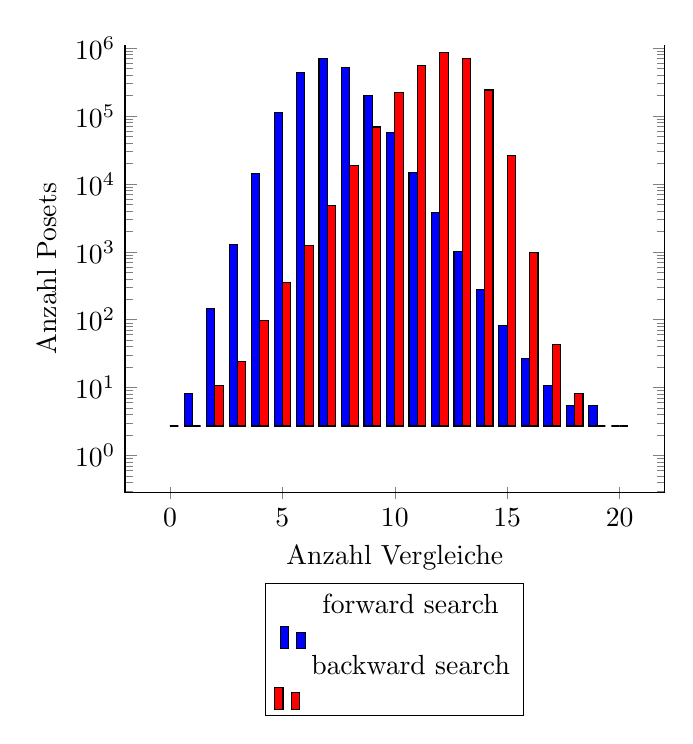
\begin{tikzpicture}
  \begin{axis}[
      ybar,
      ymode=log,
      axis x line = bottom,%x-Achse nur unten
      enlarge x limits = .1,%x-Achse erweitern
      x axis line style = {-},%kein Pfeil
      bar width=3pt,
      ylabel={Anzahl Posets},
      xlabel={Anzahl Vergleiche},
      % legend cell align=left,
      % legend pos=outer north east,
      legend style={at={(0.5,-0.2)},anchor=north}, % draw=none
    ]
    \addlegendentry{forward search}
    \addplot[fill=blue,shift={(1pt, 0)}] table {
        x y
        0  0
        1  3
        2  54
        3  467
        4  5226
        5  42082
        6  162696
        7  260188
        8  191555
        9  74694
        10 21096
        11 5470
        12 1387
        13 375
        14 103
        15 30
        16 10
        17 4
        18 2
        19 2
        20 1
      };
    \addlegendentry{backward search}
    \addplot[fill=red,shift={(-1pt, 0)}] table {
        x y
        20 1
        19 1
        18 3
        17 16
        16 365
        15 9509
        14 88920
        13 259021
        12 318522
        11 202924
        10 82456
        9  25372
        8  6848
        7  1770
        6  461
        5  130
        4  36
        3  9
        2  4
        1  1
        0  1
      };
  \end{axis}
\end{tikzpicture}
  \centering
  \caption{Anzahl Posets vs. Anzahl Vergleiche für $n=12, i=5$ (rot: Rückwärtssuche, blau: Vorwärtssuche)}
  \label{fig:backward_forward_count_12_5}
\end{figure}

\begin{figure}[h!]
  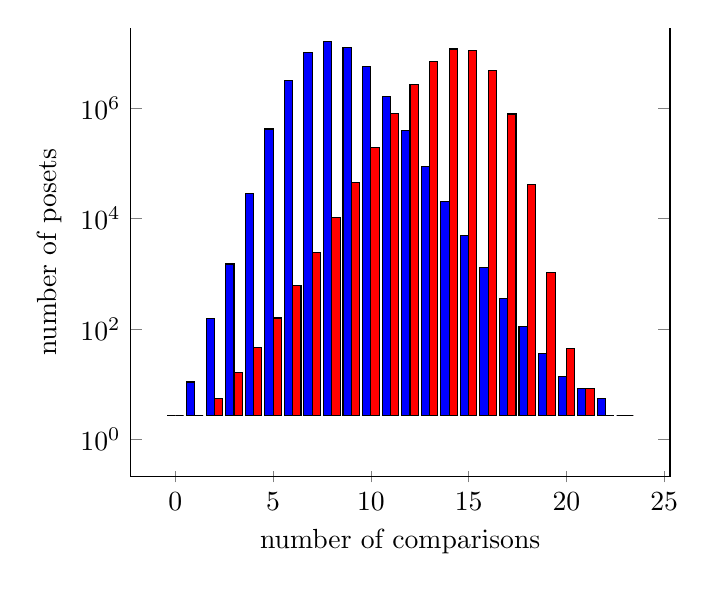
\begin{tikzpicture}
  \begin{axis}[
      ybar,
      ymode=log,
      axis x line = bottom,%x-Achse nur unten
      enlarge x limits = .1,%x-Achse erweitern
      x axis line style = {-},%kein Pfeil
      bar width=3pt,
      ylabel={number of posets},
      xlabel={number of comparisons},
      % legend cell align=left,
      % legend pos=outer north east,
      % legend style={at={(0.5,-0.2)},anchor=north}, % draw=none
    ]
    % \addlegendentry{forward search}
    \addplot[fill=blue,shift={(1pt, 0)}] table {
        x y
        0  1
        1  4
        2  57
        3  552
        4  10397
        5  154828
        6  1166640
        7  3770182
        8  5941732
        9  4726819
        10 2096404
        11 604582
        12 143058
        13 32460
        14 7450
        15 1823
        16 471
        17 132
        18 41
        19 13
        20 5
        21 3
        22 2
        23 1
      };
    % \addlegendentry{backward search}
    \addplot[fill=red,shift={(-1pt, 0)}] table {
        x y
        23 1
        22 1
        21 3
        20 16
        19 381
        18 15227
        17 290138
        16 1750707
        15 4058631
        14 4368185
        13 2592437
        12 1006071
        11 291970
        10 72346
        9  16728
        8  3898
        7  893
        6  227
        5  58
        4  17
        3  6
        2  2
        1  1
        0  1
      };
  \end{axis}
\end{tikzpicture}

Treff: 11
  \centering
  \caption{Anzahl Posets vs. Anzahl Vergleiche für $n=13, i=6$ (rot: Rückwärtssuche, blau: Vorwärtssuche)}
  \label{fig:backward_forward_count_13_6}
\end{figure}

Wie in Abbildung~\ref{fig:backward_forward_count_13_6} zu sehen, durchsucht die Vorwärtssuche für $n = 13, i = 6$ die meisten Posets bei $k = 6$ Vergleichen, während die Rückwärtssuche die meisten Posets bei $k = 14$ durchsucht.
Dies ist sehr unvorteilhaft für eine bidirektionale Suche, da der Großteil des Suchraums vor dem Treffpunkt beider Suchen liegt.

% TODO: Ergebnisse der Bidirektionalen Suche vorstellen

%%%%%%%%%%%%%%%%%%%%%%%%%%%%%%%%%%%%%%%%%%%%%%%%%%%%%%%%%%%%%%%%%

\subsection{Pruning Decisions}
The minimax search algorithm explained in chapter~\ref{chapter:forward_search} allows for cutting off unpromising branches. For this means, the following strategies are applied.

\begin{enumerate}
  \item[1.]
    Use solvable-heuristic. A heuristic is employed to estimate whether a poset is solvable. If the heuristic's estimate states 'unsolvable', the branch is pruned.
    Otherwise, the search continues regularly.
  \item[2.]
    Use \texttt{current\_best}. Each call of \texttt{search\_rec} gets a maximum numbers of comparisons.
    When searching the children of a node, the limit is the best (minimal) value found so far.
\end{enumerate}

\section{Results}

\begin{table}
  \centering
  \begin{tabular}{c|cccccccc}
    $n$ & \multicolumn{8}{c}{$i$}                                    \\
        & 0                       & 1  & 2  & 3  & 4  & 5  & 6  & 7  \\ \hline
    1   & 0                                                          \\
    2   & 1                                                          \\
    3   & 2                       & 3                                \\
    4   & 3                       & 4                                \\
    5   & 4                       & 6  & 6                           \\
    6   & 5                       & 7  & 8                           \\
    7   & 6                       & 8  & 10 & 10                     \\
    8   & 7                       & 9  & 11 & 12                     \\
    9   & 8                       & 11 & 12 & 14 & 14                \\
    10  & 9                       & 12 & 14 & 15 & 16                \\
    11  & 10                      & 13 & 15 & 17 & 18 & 18           \\
    12  & 11                      & 14 & 17 & 18 & 19 & 20           \\
    13  & 12                      & 15 & 18 & 20 & 21 & 22 & 23      \\
    14  & 13                      & 16 & 19 & 21 & 23 & 24 & 25      \\
    15  & 14                      & 17 & 20 & 23 & 24 & 26 & 26 & 27 \\
  \end{tabular}
  \caption{The minimum amount of comparisons needed to select the $i+1$-th smallest of $n$}
  \label{table:num-comparisons}
\end{table}

See Table~\ref{table:num-comparisons}.


\subsection{Search evaluation}
\subsubsection{Backward search}
\subsubsection{bidirectional search}
\subsubsection{forward search}

\subsection{Algorithmic improvements}

\subsubsection{Heuristics}

We used multiple heuristics to estimate if a poset is solvable in a given number of comparisons.
These heuristics are used to reject posets, that are not solvable in the given number of comparisons.
This reduces the number of posets that need to be searched.

The first heuristic uses the number of compatible posets.
We use the fact, that the number of comparisons needed to solve a poset is less than the base two logarithm of the number of compatible posets,
to estimate if a poset is solvable.

The second heuristic searches for two elements which have not beend compared yet.
One of these two elements is maximal and has at least two elements smaller than it,
and the other element is minimal and has at least two elements greater than it.
We then construct a new poset with a comparison added, where the minimal element is smaller than the maximal.
The new poset is then searched for a solution using the forward seach described above.
If the new poset is found to be solvable in the given number of comparisons, we estimate that the original poset is also solvable.
If the new poset is not solvable, we estimate the original is not solvable either.
This heuristic can be slightly improved by maximising the number of elements smaller than the maximal element and greater than the minimal element.

\subsubsection{Triangular Adjacency Matrix}
Storing an adjacency matrix for a poset of size $n$ takes $n^2 - n$ bits, one for each possible relation.
The diagonal does not need to be stored, as an element can not be smaller than itself.

By canonifying the poset, the elements can be sorted in a way such that each element is not smaller than any element before it.
This property can be used to reduce the adjacency matrix to a triangular matrix, which can then be stored using $\frac{n^2 - n}{2}$ bits.
It can also simplify some algorithms, for example calculating the number of compatible posets.

\subsubsection{Multithreading}

\section{Conclusion}
We found a better solution hooray!
These are points we'd like to take into account for further research


\appendices
\section{Proof of the First Zonklar Equation}
Appendix one text goes here.
\section{}
Appendix two text goes here.


\ifCLASSOPTIONcompsoc
  \section*{Acknowledgments}
\else
  \section*{Acknowledgment}
\fi


The authors would like to thank...

FMI
Hardware
Florian Stober
Armin weiß

\ifCLASSOPTIONcaptionsoff
  \newpage
\fi


\bibliographystyle{IEEEtran}
\bibliography{biblio.bib}
\end{document}